% Copyright 2004 by Till Tantau <tantau@users.sourceforge.net>.
%
% In principle, this file can be redistributed and/or modified under
% the terms of the GNU Public License, version 2.
%
% However, this file is supposed to be a template to be modified
% for your own needs. For this reason, if you use this file as a
% template and not specifically distribute it as part of a another
% package/program, I grant the extra permission to freely copy and
% modify this file as you see fit and even to delete this copyright\usecolortheme[named=CornellRed]{structure}
% notice. 

\documentclass[xcolor = dvipsnames]{beamer}
\usefonttheme{serif}
\usepackage{graphicx, caption}

\usepackage{subcaption}
\usepackage{amsmath,amscd, amsthm, mathrsfs, amssymb, esint}
\usepackage{graphics}
\usepackage{mathtools}
\usepackage{biblatex}

\useoutertheme{miniframes} % Alternatively: miniframes, infolines, split
\useinnertheme{circles}

\definecolor{CornellRed}{RGB}{179, 27, 27} % UBC Blue (primary)

\usecolortheme[named=CornellRed]{structure}
% There are many different themes available for Beamer. A comprehensive
% list with examples is given here:
% http://deic.uab.es/~iblanes/beamer_gallery/index_by_theme.html
% You can uncomment the themes below if you would like to use a different
% one:
%\usetheme{AnnArbor}
%\usetheme{Antibes}
%\usetheme{Bergen}
%\usetheme{Berkeley}
%\usetheme{Berlin}
%\usetheme{Boadilla}
%\usetheme{boxes}
%\usetheme{CambridgeUS}
%\usetheme{Copenhagen}
%\usetheme{Darmstadt}
%\usetheme{default}
%\usetheme{Frankfurt}
%\usetheme{Goettingen}
%\usetheme{Hannover}
%\usetheme{Ilmenau}
%\usetheme{JuanLesPins}
%\usetheme{Luebeck}
%\usetheme{Madrid}
%\usetheme{Malmoe}
%\usetheme{Marburg}
%\usetheme{Montpellier}
%\usetheme{PaloAlto}
%\usetheme{Pittsburgh}
\usetheme{Rochester}
%\usetheme{Singapore}
%\usetheme{Szeged}
%\usetheme{Warsaw}
\usepackage{amsmath,amscd, amsthm, mathrsfs, amssymb, esint}
\usepackage{graphicx}
\usepackage{float}

\usepackage{subcaption}
%\usepackage{subfig}
\usepackage{mathtools}
%\DeclarePairedDelimiter\abs{\lvert}{\rvert}


\makeatother
\usepackage{array}
\usepackage{booktabs}

\newcommand{\lap}{\Delta}





\setbeamersize{text margin left=5mm,text margin right=5mm} 
\title{Chebyshev and Sobolev Orthogonal Polynomials}

% A subtitle is optional and this may be deleted


\author{Max Jiang, Tian Lan, Shashank Sule, Sreeram Venkat, Xiaoduo Wang\\Advisors: Robert Strichartz and Kasso Okoudjou}
% - Give the names in the same order as the appear in the paper.
% - Use the \inst{?} command only if the authors have different
%   affiliation.

\institute{Cornell SPUR 2019: Analysis on Fractals}% (optional, but mostly needed)

% - Use the \inst command only if there are several affiliations.
% - Keep it simple, no one is interested in your street address.

\date{\today}
% - Either use conference name or its abbreviation.
% - Not really informative to the audience, more for people (including
%   yourself) who are reading the slides online

%\subject{MATH 320}
% This is only inserted into the PDF information catalog. Can be left
% out. 

% If you have a file called "university-logo-filename.xxx", where xxx
% is a graphic format that can be processed by latex or pdflatex,
% resp., then you can add a logo as follows:

% \pgfdeclareimage[height=0.5cm]{university-logo}{university-logo-filename}
% \logo{\pgfuseimage{university-logo}}

% Delete this, if you do not want the table of contents to pop up at
% the beginning of each subsection:
\AtBeginSubsection[]
{
  \begin{frame}<beamer>{Outline}
    \tableofcontents[currentsection,currentsubsection]
  \end{frame}
}

% Let's get started
\begin{document}

\begin{frame}
  \titlepage
\end{frame}

\begin{section}{Introduction}
\begin{frame}{Preliminaries}
\begin{itemize}
    \item Let $V_0 = \{q_0, q_1, q_2\} \in \mathbb{R}^2$ and $F_i(x) = \frac{1}{2}(x+q_i)$ for $i=0,1,2$. Then $$SG = \overline{\bigcup_{m=1}^{\infty}\bigcup_{|w|=m}F_w(V_0)}$$
    \pause
    \item We work on the finite graph approximation $V_m = \bigcup_{|w|=m}F_{w}(V_0)$
    \begin{figure}
        \centering
        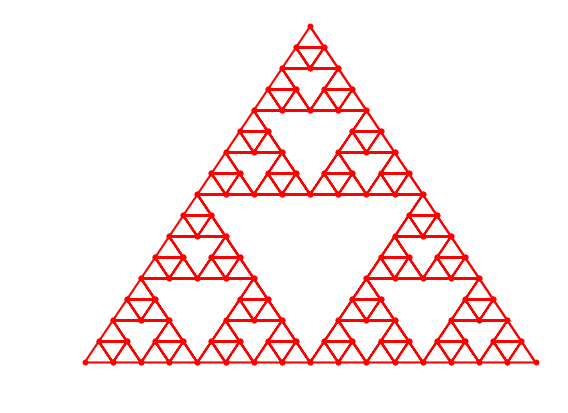
\includegraphics[width=0.45\linewidth]{Final_presentation/images/V4.png}
        \caption{$V_4$}
        \label{fig:V4}
    \end{figure}
\end{itemize}
\end{frame}

\begin{frame}{Preliminaries}
    \begin{itemize}
        \item Let $u: SG \mapsto \mathbb{R}$. Then the \textbf{Laplacian} $\Delta_{\mu}$ is defined as
        $$  \Delta_{\mu}u(x) = \frac{3}{2}\lim_{m \to \infty}5^m\Delta_mu(x)$$
        \pause
        \item $G: SG \times SG \mapsto R$ is called \textbf{Green's Function} where
        $$ -\Delta u = f, u|_{V_0} = 0 \iff u(x) = \int_{SG}G(x,y)f(y)\,d\mu$$
        \pause
        \item $\partial_nu(q_i)$ is the \textbf{normal derivative} of $u$ at $q_i$ where
        $$ \partial_nu(q_i) = \lim_{m \to \infty}\Big(\frac{5}{3}\Big)^m(2u(q_i) - u(F^{m}_{i+1}q_i) - u(F^{m}_{i-1}q_i))$$
        \pause
        \item $\partial_Tu(q_i)$ is the \textbf{tangential derivative} of $u$ at $q_i$ where
        $$ \partial_{T}u(q_i) = \lim_{m\to\infty}5^m(u(F^{m}_{i+1}q_i) - u(F^{m}_{i-1}q_i))$$
        
    \end{itemize}
\end{frame}
\begin{frame}{Polynomials on SG: The space $\mathcal{H}_j$}
    \begin{itemize}
        \item Let $f: SG \mapsto \mathbb{R}$. Then $f$ is a $j$-degree polynomial iff\\
        $\Delta^{j+1}f = 0$ and $\Delta^{j}f\neq 0$, i.e $f$ is $j$-harmonic but not ($j-1$)-harmonic. 
        \pause
        \item The space of polynomials with degree $\le j$ is denoted $\mathcal{H}_{j}$
        \pause
        \item Let $f \in \mathcal{H}_j$. Then $f$ is determined uniquely by the values $(f(q_0), f(q_1), f(q_2), \Delta f(q_0), \Delta f(q_1), \ldots, \Delta^jf(q_2))$
        \pause
        \item dim($\mathcal{H}_j$) = $3j + 3$
        \pause
        \item A natural basis for $\mathcal{H}_{j}$ is the family of functions $\{f_{nk}\}$ where 
        $$ \Delta^{m}f_{nk}(q_i) = \delta_{mn}\delta_{ki}$$
        \pause
        \item For example, the three harmonic functions $h_i$ where $h_i(q_j) = \delta_{ij}$ form a basis for $\mathcal{H}_0$
    \end{itemize}
\end{frame}

\begin{frame}{Polynomials on SG: The monomial basis}
    \begin{itemize}
        \item We want to mimic the case on $I = [0,1]$ where we can expand a function as a Taylor series in terms of basis functions where we use derivative information at one point. 
        \pause
        \item For example, for harmonic functions, we have the following basis $\{P_{0k}\}$ where the tuple of values $(u(q_0), \partial_nu(q_0), \partial_Tu(q_0)) = e_k$:
        $$ P_{01} = h_0 + h_1 + h_2 \hspace{0.35in} P_{02} = -\frac{1}{2}(h_1 + h_2) \hspace{0.35in} P_{03} = \frac{1}{2}(h_1 - h_2) $$
         If $f \in \mathcal{H}_0$ then $f = f(q_0)P_{01} + \partial_nf(q_0)P_{02} + \partial_Tf(q_0)P_{03}$
        \pause
        \item We introduce the following basis $\{P_{jk}\}$ where
        \begin{align*}
            \Delta^nP_{jk}(q_0) &= \delta_{nj}\delta_{k1}\\
            \Delta^n\partial_nP_{jk}(q_0) &= \delta_{nj}\delta_{k2}\\
            \Delta^n\partial_TP_{jk}(q_0) &= \delta_{nj}\delta_{k3}\\
        \end{align*}
        This is known as the \textbf{monomial basis}. 
    \end{itemize} 
\end{frame}


\begin{frame}{Polynomials on SG: The monomial basis}
    \begin{figure}[H]
        \centering
        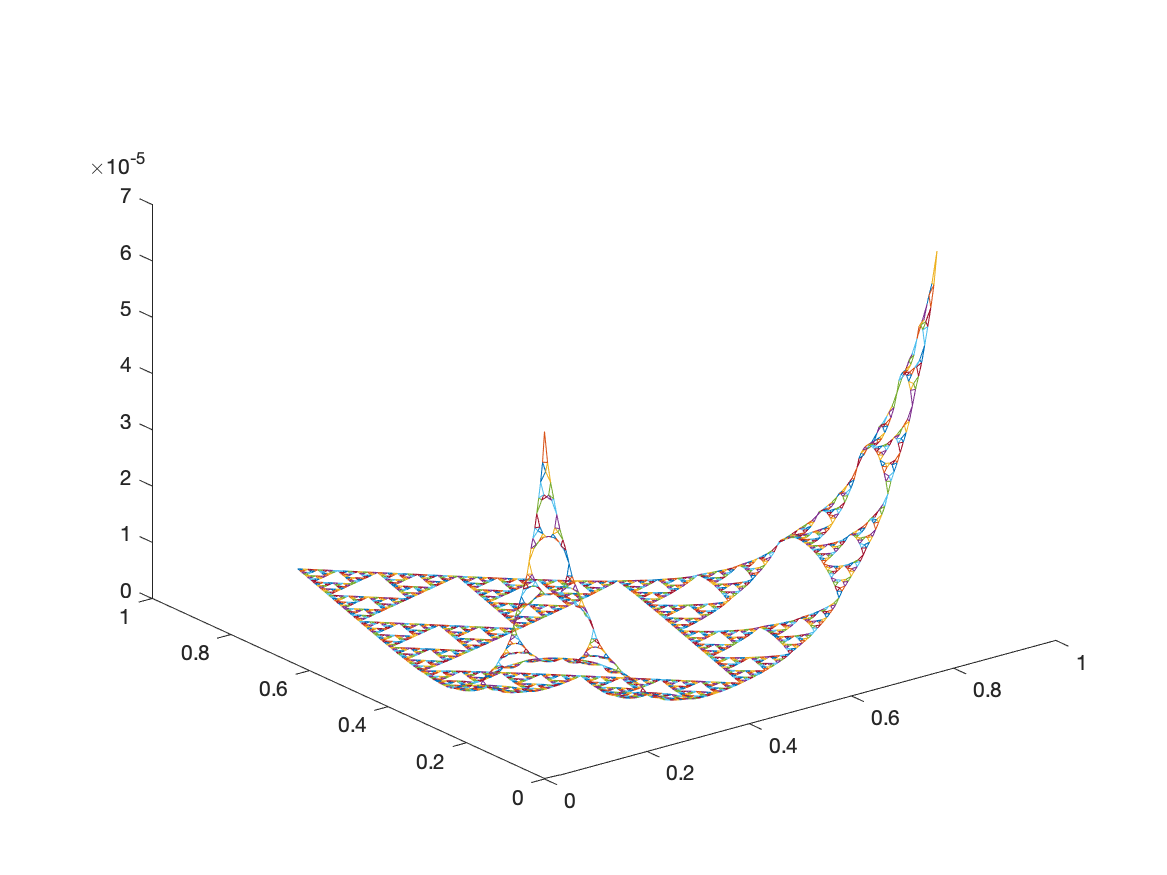
\includegraphics[width=0.75\linewidth]{monomial3_1.png}
        \caption{$P_{31}$}
    \end{figure}
\end{frame}

\begin{frame}{Polynomials on SG: The monomial basis}

    \begin{figure}[H]
        \centering
        
        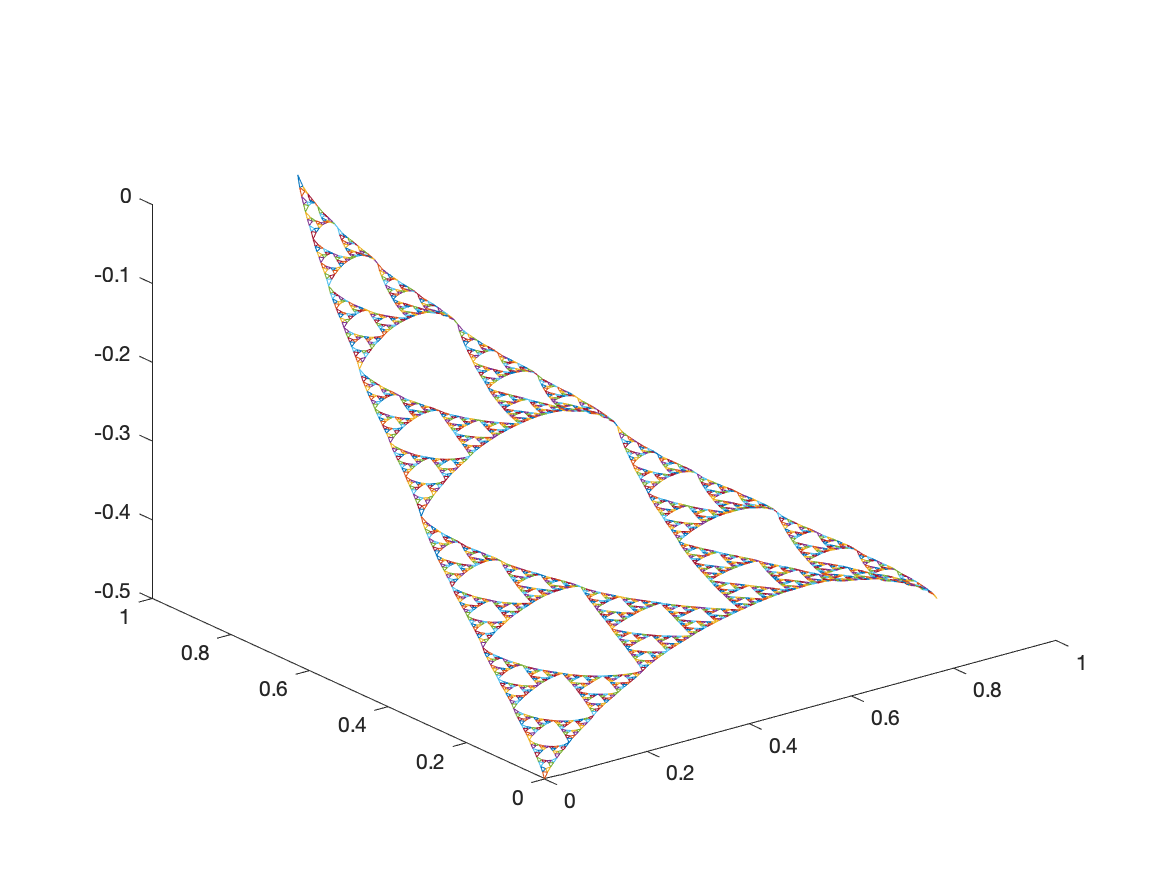
\includegraphics[width=0.75\linewidth]{monomial0_2.png}
        \caption{$P_{02}$}
        
    \end{figure}
    
\end{frame}

\begin{frame}{Polynomials on SG: The monomial basis}

    \begin{figure}[H]
        \centering
        
        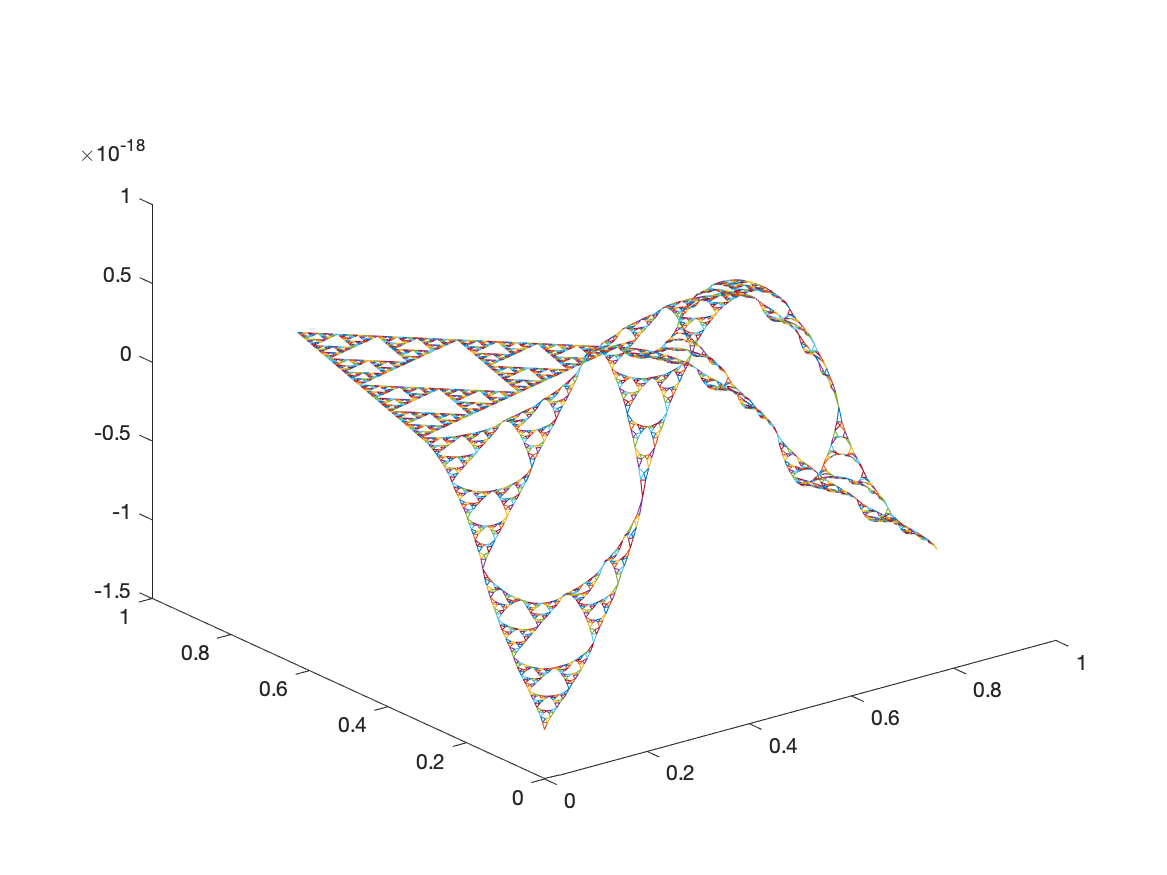
\includegraphics[width=0.75\linewidth]{monomial8_2.png}
        \caption{$P_{82}$}
        
    \end{figure}
    
\end{frame}

\begin{frame}{Polynomials on SG: The monomial basis}
    \begin{figure}[H]
        \centering
        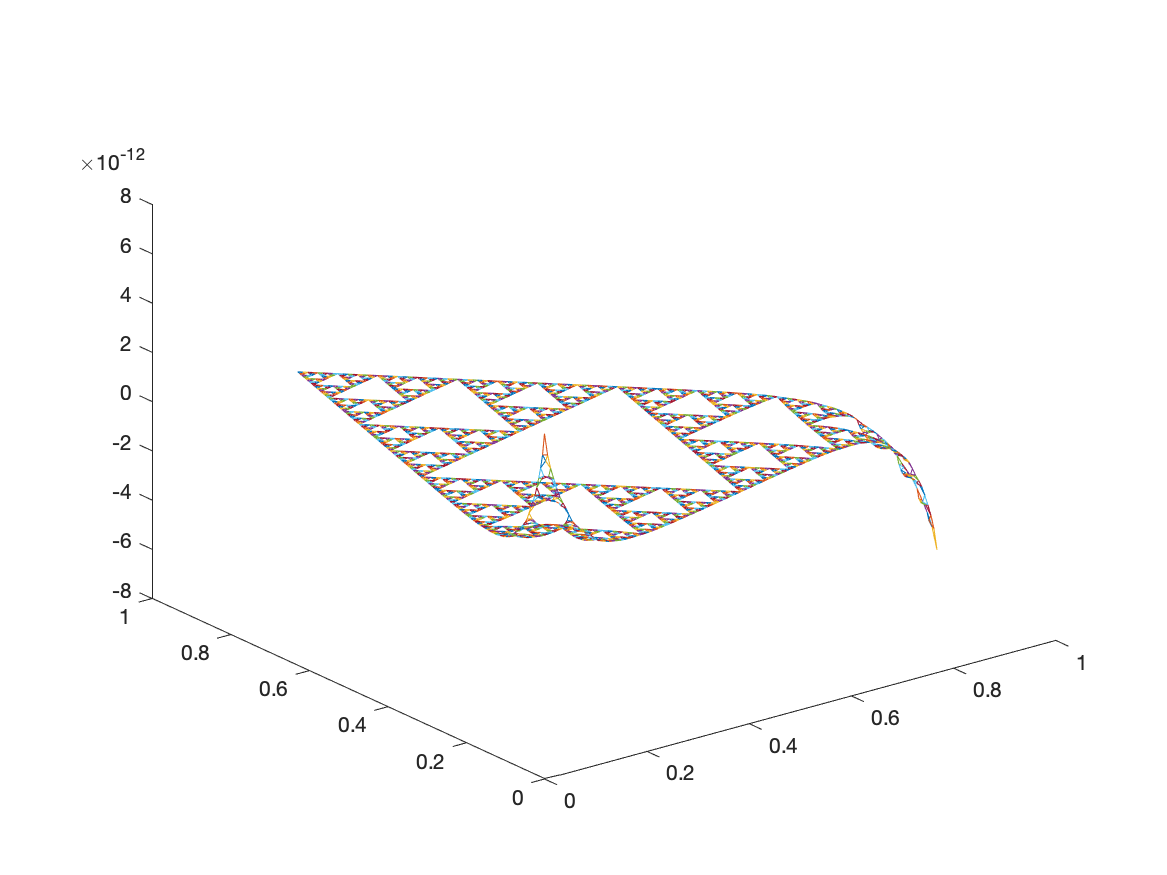
\includegraphics[width=0.75\linewidth]{monomial5_3.png}
        \caption{$P_{53}$}
    \end{figure}
\end{frame}

\begin{frame}{Polynomials on SG: The monomial basis}
    \begin{itemize}
        \item Note that $P_{j1}$ and $P_{j2}$ are symmetric across the line through $q_0$ and $F_1q_2$ and $P_{j3}$ is anti-symmetric. We thus refer to them as the $\textit{symmetric}$ and $\textit{anti-symmetric}$ families. 
        \pause
        \item Using the monomial basis, we define can functions as power series expansions:
        $$ f = \sum_{n=0}^{\infty}\sum_{k=1}^{3}c_{nk}P_{nk}(x)$$
        If $|c_{nk}| \leq Mr^{n}$ for some $r
        < \lambda_2$, the power series converges uniformly. We call such functions \textbf{entire analytic}.
    \end{itemize}
    
\end{frame}

\begin{frame}{Orthogonal polynomials}
    \begin{itemize}
        \item The space of polynomials on $\mathbb{R}$, denoted $P(\mathbb{R})$ can be endowed with the following inner product: 
        $$ \langle f,g \rangle = \int_{\mathbb{R}}f(x)g(x)w(x)\,dx$$
        where $w(x) \in L^1(\mathbb{R})$
        \pause
        \item Given an inner product space, we can generate an \textit{orthogonal basis} using the Gram-Schmidt process. The resulting polynomials are called $\textit{orthogonal polynomials}$
        \pause
        \item Common examples for $w(x)$ include $\chi_{[-1,1]}(1-x)^\alpha(1+x)^\beta$, $e^{-x^2}$, and $\chi_{[0,\infty)}e^{-x}$
    \end{itemize}
\end{frame}
\end{section}

\begin{frame}{Orthogonal Polynomials}
    \begin{table}[]
        \centering
        \begin{tabular}{cc}
             
             $w(x)$ & Name \\
             \hline
             \hline
             $\chi_{[-1,1]}(1-x)^\alpha(1+x)^\beta$ & Jacobi \\
             
             $e^{-x^2}$ & Hermite \\
             
             $\chi_{[0,\infty)}e^{-x}$ & Laguerre \\
             
        \end{tabular}
        \caption{Classical orthogonal polynomials on $\mathbb{R}$}
        \label{tab:Classical polys}
    \end{table}
    \pause
    There are two special cases of Jacobi polynomials: 
    \begin{itemize}
        \item When $\alpha = \beta = 0$, they are known as the \textbf{Legendre polynomials}. In this case the inner product is the standard $L^2$ product on $[-1,1]$: $\langle f, g \rangle_{L^2} = \int_{-1}^{1}fg\,dx$.
        \item When $\alpha = \beta = 1/2$, they are known as the \textbf{Chebyshev polynomials}. Here the weight function is $\sqrt{1-x^2}$ 
    \end{itemize} 
    
\end{frame}

\begin{frame}{Orthogonal Polynomials}
    Classical orthogonal polynomials, denoted $P_n$ satisfy the following properties:
    \pause
    \begin{enumerate}
        \item $Q(x)P''_n(x) + L(x)P'_n(x) + \lambda_nP_n(x) = 0$ where $Q,L$ are polynomials and $\lambda_n \in \mathbb{R}$
        \pause
        \item $P_n(x) = \frac{1}{e_nw(x)}\dfrac{d^n}{dx^n}(w(x)[Q(x)]^n)$ This is known as the \textbf{Rodrigues' formula}.
        \pause
        \item Two term recurrence: $a_nxP_{n}(x) = b_nP_{n+1}(x) + c_nP_{n-1}(x)$
    \end{enumerate}
    \pause
    Okoudjou et. al (2012) found the Legendre polynomials on SG (the orthogonal polynomials with respect to the $L^2$ inner product). 
    We will study orthogonal polynomials with respect to other inner products, usually involving the Laplacian. These will be known as the $\textbf{Sobolev}$ inner products. 
\end{frame}%\endShashank

\section{Sobolev Orthogonal Polynomials}
\begin{frame}{Origin of Sobolev Orthogonal Polynomials}
    \begin{itemize}
        \item Idea (Lewis): Given $f \in L^2[-1,1]$, find polynomial $g$ with deg $g\le n$ such that $g$ minimizes the quantity $\|f-g\|_{H}$, where $\|h\|_{H}^2:=\int (h^2(x)dx+h'{^2}(x))dx$
        \pause
        \item Solution: $\widetilde g=\sum\limits^{n}_{i=0} \langle f,e_i\rangle_H\,e_i$, $\{e_i\}$ orthonormal basis
        \pause
        \item Core idea: Approximate a function by polynomials as “close” as possible.

    \end{itemize}
\end{frame}

% Section and subsections will appear in the presentation overview
% and table of contents.
\begin{frame}{Generalization to SG}
\begin{itemize}
\item Unless specified we will consider the Sobolev inner product $\langle f,g\rangle_H:=\langle f,g\rangle_{L^2}+\lambda\langle \lap f,\lap g\rangle_{L^2}$ for some nonnegative 
constant $\lambda$, where $\langle f,g\rangle_{L^2}:=\int fg\,d\mu$ for a regular Borel probability measure $\mu$ that is symmetric with respect to the line passing through $q_0$ and the midpoint of the side opposing $q_0$\pause
\item the monic Sobolev polynomials $\{S_{nk}(x;\lambda)\}_{n=0}^{\infty}$(For simplicity, write as $\{S_{n}\}_{n=0}^{\infty}$), is obtained by Gram-Schmidt Process.

\end{itemize}
\end{frame}
\begin{frame}{Recurrence (Case 1: k=2 or 3)}
\textbf{Theorem}: When $k = 2$ or $3$ we have the following recurrence relation for $n\geq-1$, where $S_{-1}:=0$.
$$S_{n+2} - a_nS_{n+1}-b_nS_n = f_{n+2}$$
where 
$f_{n+2} := \mathcal{G}(p_{n+1})$, and $\mathcal{G}(g)(x):=-\int_{SG}G(x,y)g_{n+1}(y)dy$,\\ $$a_n = -\frac{\langle f_{n+2}S_{n+1}\rangle_H}{\|S_{n+1}\|_H^2}$$ $$b_n = -\frac{\langle f_{n+2},S_{n}\rangle_H}{\|S_{n}\|_H^2}$$

    
\end{frame}
\begin{frame}{Recurrence: (Case 1: k=2 or 3)}
    \textbf{Remark}: When $k = 2$ or $3$, the same recursive relation is still valid if we replace the Sobolev inner product by $\langle f,g\rangle_H:=$ $$\langle f,g\rangle_{L^2}+\lambda_1 \langle \lap f,\lap g\rangle_{L^2}+\lambda_2\,\varepsilon(f,g)+$$ $$[f(q_0)\,f(q_1)\,f(q_2)] M [g(q_0)\,g(q_1)\,g(q_2)]^T$$ for nonnegative constants $\lambda_1$ and $\lambda_2$, positive semidefinite $3\times3$ matrix $M$
\end{frame}
\begin{frame}{Recurrence (Case 1: k=2 or 3)}
    \textbf{Corollary}: When $k =2$ or $3$, $(a_n, b_n)$ is the unique solution to the system $a_n S_{n+1}(q_1)+b_nS_n(q_1)=S_{n+2}(q_1)$ and $a_n \partial_n S_{n+1}(q_1)+b_n\partial_n S_n(q_1)=\partial_n S_{n+2}(q_1)$. In particular, the matrix $\left[\begin{matrix}
S_{n+1}(q_1)&S_n(q_1)\\
\partial_n S_{n+1}(q_1) &\partial_n S_n(q_1)
\end{matrix}\right]$ is non-singular for any integer $n\geq 0$.

\end{frame}
\begin{frame}{Recurrence: (Case 1: k=2 or 3)}
   \begin{itemize} \item\textbf{Asymptotics}: Firstly, We are interested in the case when $\lambda\rightarrow\infty$.
   \pause
   \item
\textbf{Estimates}: $\|S_n\|_{H}^2=\Theta (\lambda)$, $|a_n|=O(\lambda^{-1})$, $|b_n|=\Theta(\lambda^{-1})$
$$\|\lap S_n\|_{L^2}^2\le \lambda^{-1}\|G\|_{L^2}^2\|p_{n-1}\|_{L^2}^2+\|p_{n-1}\|_{L^2}^2 $$
$$\|S_n\|_{L^{\infty}}\le C(1+\lambda^{-\frac12})\|p_{n-1}\|_{L^2}$$ (C is independent of $n$ and $\lambda$)
\end{itemize}
\end{frame}
\begin{frame}{Recurrence (Case 1: k=2 or 3, Asymptotic)}
    \textbf{Theorem}: Suppose $k=2$ or $3$. Then for any $n\ge3$, $S_n(x;\lambda)$ converges to $f_n$ uniformly in $x$ as $\lambda\rightarrow\infty$. Consequently $\lap S_n\rightarrow p_{n-1}$ uniformly as $\lambda\rightarrow\infty$. Also, 

$$\lambda(S_n(\lambda)-f_n)\rightarrow-\frac{\langle f_n,f_{n-1}\rangle_{L^2}}{\|p_{n-2}\|_{L^2}^2}f_{n-1}-\frac{\|p_{n-1}\|_{L^2}^2}{\|p_{n-3}\|_{L^2}^2}f_{n-2}$$ uniformly in $x$ as $\lambda\rightarrow\infty$

\end{frame}
\begin{frame}{Recurrence (Case 2: k=1)}
    \begin{itemize}
        \item More complicated!\pause
        \item Requires a conjecture: $\partial_n f_t(q_0)\neq 0$, where $f_t:=\mathcal{G} (p_{t-1})$.\pause
\item \textbf{Theorem}: Let $S_{-1}:=0$, k=1, $f_{n+2}= \mathcal{G}(p_{n+1})$ and suppose that $\partial_n f_{n+2}(q_0)\neq 0$, then $S_{n+3}-a_nS_{n+2} - b_nS_{n+1}-c_nS_n = f_{n+3}+d_nf_{n+2}$, The matrix\begin{align}
     \begin{bmatrix}
    S_{n+2}(q_1)&S_{n+1}(q_1)&S_{n}(q_1)\\
    \partial_n S_{n+2}(q_1) &\partial_n S_{n+1}(q_1)&\partial_n S_{n}(q_1)\\
    S_{n+2}(q_0)&S_{n+1}(q_0)&S_{n}(q_0)
    \end{bmatrix} 
\end{align}
is non-singular.

    \end{itemize}
\end{frame}
\begin{frame}{Recurrence (Case 2: k=1, Asymptotics)}
    \textbf{Theorem}: Assume the normal derivative conjecture is true. Then there exists a sequence of monic polynomials $\{g_n\}_{n=0}^{\infty}$ independent of $\lambda$ such that for any $n\ge0$, $deg\, g_n=n$, $S_n$ converges uniformly in $x$ to $g_n$. And $g_{n+3}+d_ng_{n+2}=f_{n+3}+d_nf_{n+2}$ for any $n\ge 1$. For the basic cases, $g_0=p_0$, $g_1=p_1$, $g_{2}+d_{-1}g_{1}=f_{2}+d_{-1}f_{1}-\frac{\langle f_2+d_{-1}f_1,{g_0}\rangle_{L^2}}{{\|g_0\|_{L^2}^2}}g_{0}$, and 
$g_{3}+d_{0}g_{2}=f_{3}+d_{0}f_{2}-\frac{\langle f_3+d_{0}f_2,{g_0}\rangle_{L^2}}{{\|g_0\|_{L^2}^2}}g_{0}$. Moreover, for any $\alpha<1$, $n\ge0$, $\lim\limits_{\lambda \rightarrow\infty}\lambda^\alpha(S_n(\lambda)-g_n)=0$ uniformly in $x$.

\end{frame}
\begin{frame}{Recurrence: Generalization (k=2 or 3)}
\begin{itemize}
    \item Consider the inner product: $\langle f,g\rangle_{H^m} = \sum\limits_{l = 0}^m \lambda_l\int_{SG}\lap^lf\lap^lg\,d\mu$
    \pause
\item \textbf{Theorem}: $S_{n+m+1} - \mathcal{F}_{n+m+1} - \sum\limits_{l = 0}^{2m-1}a_{n, l}S_{n+m-l} = 0$, where $\mathcal{F}_{n+m+1} := \mathcal{G}^mp_{n+1}$
\pause
\item \textbf{Remark}: It is still true if we consider $\langle f,g\rangle_{H^m}= 
\sum\limits_{l = 0}^m \lambda_l\int_{SG}\lap^lf\lap^lg\,d\mu+\sum\limits_{l=0}^{m-1}\beta_l\,\varepsilon(\lap^l f,\lap^l g)+\nonumber
\sum\limits_{l=0}^{m-1}[\lap ^lf(q_0)\,\lap ^lf(q_1)\,\lap ^lf(q_2)] M_l [\lap ^lg(q_0)\,\lap ^lg(q_1)\,\lap ^lg(q_2)]^T$, where $M_l$ are positive definite $3\times 3$ matrices.

\end{itemize}
    
\end{frame}
\begin{frame}{Recurrence: Generalization (k=2 or 3)}
Asymptotic: we consider the case $\lambda_m\rightarrow\infty$, and the other parameters are bounded.\\
\textbf{Theorem}: Suppose $k=2$ or $3$, and there exists $M>0$ such that $\lambda_l\le M$ for any $l<m$. Then for any $n\ge 2m+1$, we have$$\|S_n-\mathcal{F}_n\|_{L^2}\le
   C(n,M,m,\mu)\lambda_m^{-1}$$ Consequently, $\lim\limits_{\lambda_m\rightarrow\infty}\|\lap^i S_n-\mathcal{G}^{m-i}p_{n-m}\|_{L^\infty}\rightarrow 0$ for any $0\le i\le m$.


\end{frame}
\begin{frame}{Zeros: Continuous functions}
    \textbf{Theorem} (Topological result): Let $f$ be a continuous function defined on $SG$. Suppose $f$ has finitely many zeros. Let $Z_0$ be the intersection of zero set $Z$ of $f$ and $V^*$. Then for any connected component $D$ in $SG\setminus Z_0$, either $f\ge0$ on $D$ or $f\le0$ on $D$.

\end{frame}
\begin{frame}{Zeros: Entire Analytic functions}
    \textbf{Theorem}: Suppose $f(x)=\sum\limits^\infty_{j=t_1}c_{j1}P_{j1}^{(0)}(x)+\sum\limits^\infty_{j=t_2}c_{j2}P_{j2}^{(0)}(x)+\sum\limits^\infty_{j=t_3}c_{j3}P_{j3}^{(0)}(x)$ where $c_{t_1,1}$, $c_{t_2,2}$ and $c_{t_3,3}$ are nonzero and has zero set $Z$. 
Then\begin{enumerate} \item$Z$ is compact and nowhere dense in $SG$. \pause
\item If $ t_3<t_1-1$ and $t_3<t_2$, then $f$ has infinitely many zeros that has limit point $q_0$. Moreover, suppose the conjecture $P_{j1}>0$ is true, $t_1\le t_2$ and $t_1\le t_3$. Then $q_0$ has a neighborhood $U$ such that $Z\cap U\subset\{q_0\}.$
\end{enumerate}

\end{frame}

\begin{frame}{Zeros of OPs}

How many zeros do the Orthogonal Polynomials have?


    \begin{figure}[H]
        \centering
        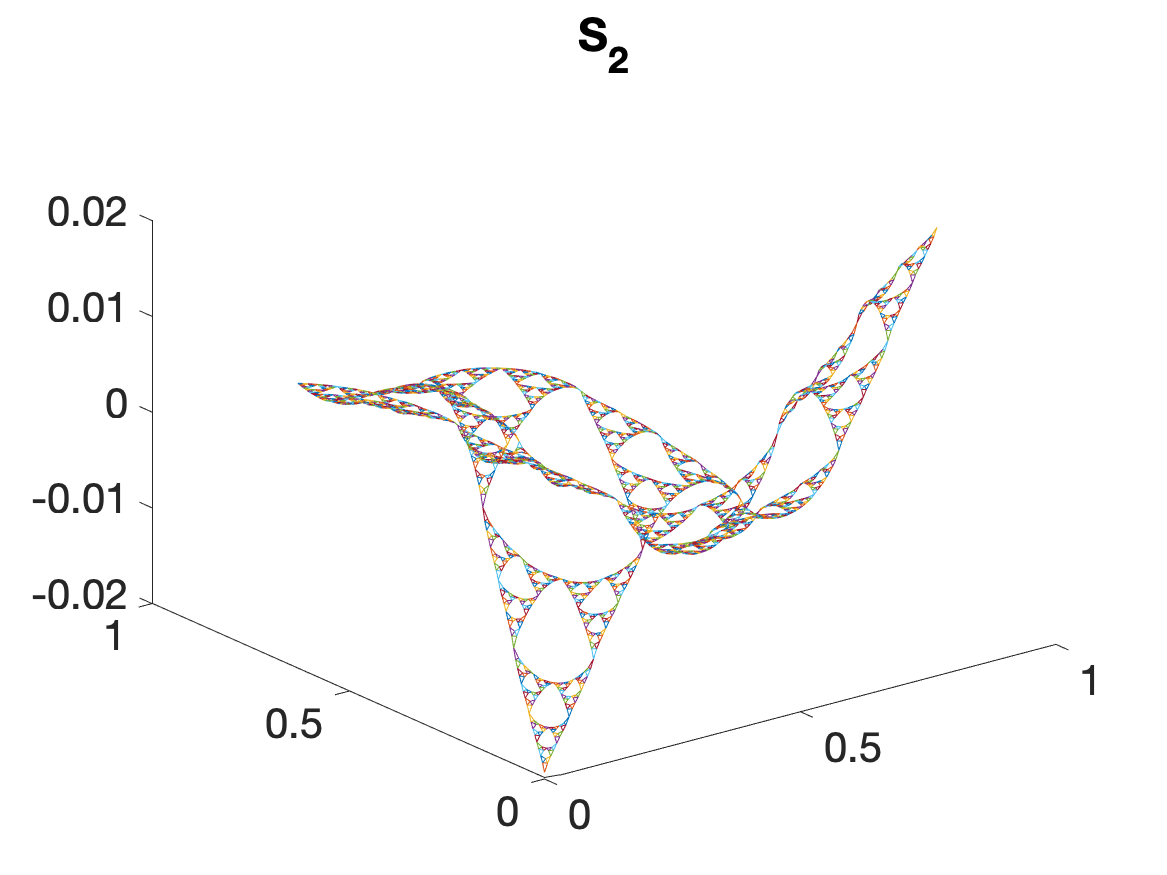
\includegraphics[width=0.7\linewidth]{images/H1AntisymOPs0_23/SAntiSym2.png}
        \caption{Antisymmetric Sobolev OP of Degree 2}
        \label{fig:S_5}
    \end{figure}
\end{frame}

\begin{frame}{Counting Zeros}
    \begin{figure}[H]
        \centering
        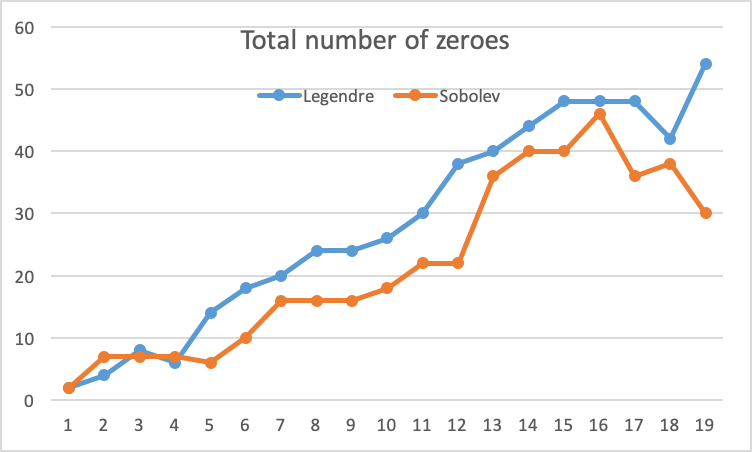
\includegraphics[width=0.7\linewidth]{images/TotalZeroes.png}
        \caption{Edge Zeros of Orthogonal Polynomials}
        \label{fig:zeros}
    \end{figure}
    
    Notice that some polynomials have more than $3n + 3$ zeros...
\end{frame}

\begin{frame}{Polynomial Interpolation and Quadrature on SG}
Questions:

\begin{itemize}
    \item Can we use polynomials (orthogonal or otherwise) to accurately interpolate functions?
    \item Can we obtain an analog of Gauss-Legendre quadrature on SG?
    \item Can we develop an algorithm for polynomial quadrature on SG and determine error estimates for it?
\end{itemize}
    
\end{frame}

\begin{frame}{Interpolation}
    \begin{itemize}
        \item Polynomials of degree $n$ can have more than $3n+3$ zeros on SG.
        \item We need to establish the invertibility of 
        
        $$
           M_n = \begin{bmatrix}
            P_{1}(x_1) & P_{1}(x_{2}) & \dots & P_{1}(x_{3n+3})\\
            \vdots & \vdots & \ddots & \vdots \\
            P_{3n+3}(x_{1}) & P_{3n+3}(x_{2}) & \dots & P_{3n+3}(x_{3n+3})
            \end{bmatrix}
        $$
    \end{itemize}
    
\end{frame}

\begin{frame}{Interpolation}
    If we choose a rotationally symmetric set of points, the interpolation matrix $M_n$ becomes circulant-block. This enables us to prove the invertibility of $M_2$. 
    \begin{figure}[H]
        \centering
        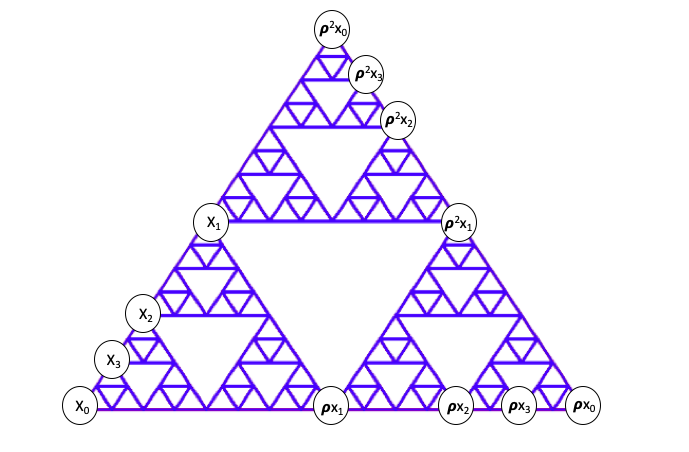
\includegraphics[width=.65\linewidth]{Final_presentation/images/Samplings.png}
        \caption{Interpolation Set for $n=3$}
        \label{fig:vortex}
    \end{figure}
\end{frame}


\begin{frame}{Interpolation}
    \begin{table}[H]
        \centering
        \begin{tabular}{c|c}
        n&$|M_n|$\\
        \toprule
            1&-1.744e-06\\
              2&1.066e-19\\
              3&-4.200e-41\\
              4&-2.058e-69\\
              5&6.788e-110\\
              6&-1.347e-163\\
              7&5.044e-232\\
              8&-4.976e-316\\
        \end{tabular}
        \caption{Determinants of $M_n$}
        \label{tab:dets}
    \end{table}
    
\end{frame}

\begin{frame}{Interpolation}
    \begin{itemize}
        \item The interpolation matrix for the $P_{jk}$ polynomials on $V_1$ points is invertible (by computation)
        \item By choosing $n+1$ points on the left side of $V_n$ along with their rotations, the interpolation matrix becomes circulant-block. These matrices are computationally invertible up to at least $n = 50$.
        \item The general case is unknown.
    \end{itemize}
\end{frame}

\begin{frame}{Quadrature}
    \begin{itemize}
        \item Gauss-Legendre quadrature on $\mathbb{R}$ requires the polynomial division algorithm on $\mathbb{R}$. However, we do not have this on SG.
        \item We have a pseudo-division algorthim on SG, but the quotient is a linear combination of powers of the Green's operator:
        $$
        \mathcal{Q}_f = \frac{1}{b_m}
        \sum\limits_{i = 0}^{n-m}c^{(i)}\mathcal{G}^{(n-m-i)}
        $$
    \end{itemize}
\end{frame}

\begin{frame}{Quadrature}
    \begin{itemize}
        \item We can try to use n-Harmonic spline quadrature, but this comes back to the interpolation problem since we need to solve
        $$
            \begin{bmatrix}
    P_{1}(x_1) & P_{1}(x_{2}) & \dots & P_{1}(x_{3n+3})\\
    \vdots & \vdots & \ddots & \vdots \\
    P_{3n+3}(x_{1}) & P_{3n+3}(x_{2}) & \dots & P_{3n+3}(x_{3n+3})
    \end{bmatrix}
    \begin{bmatrix}
    w_1\\
    \vdots\\
    w_{3n+3}
    \end{bmatrix} = 
    \begin{bmatrix}
    \int_{SG}P_{01}\\
    \vdots\\
    \int_{SG}P_{n3}
    \end{bmatrix}
    $$
    
    \end{itemize}
\end{frame}

\begin{frame}{N-Harmonic Extension: The Solution to Many Polynomial Problems on SG}
    \begin{itemize}
        \item Is there an algorithm to extend a function defined on $3n+3$ vertices of $V_n$ n-Harmonically?
        \item Given this algorithm, we have the following quadrature error estimate:
        $$
        \left|I_n^m(f) - \int_{SG}f\right|\leq c_15^{-(n+1)(m-n)}\|\Delta^{(n+1)}f\|_\infty
        $$
    \end{itemize}
\end{frame}

\begin{frame}{Outstanding Questions Regarding Polynomials on SG}
    \begin{enumerate}
        \item Is $\partial_nf_n \neq 0 \ \forall \ n$?
        \item Is $P_{j1} > 0$ except at $q_0$?
        \item Interpolation problem: Does sampling an $n$ degree polynomial on any $3n + 3$ points uniquely determine the polynomial? 
    \end{enumerate}
    Questions 2 and 3 can be solved given an n-Harmonic Extension Algorithm.
\end{frame}

\section{Extremal Points of Polynomials}
\begin{frame}{Extremal Points of Polynomials}
    \pause
    Definition of local extrema:
    \begin{enumerate}
        \item For a function $u$ defined on SG and $x\in SG$, we say that $x$ is a \textbf{local maximum (minimum)} of $u$ if $\exists$ neighborhood $U$ s.t. $x\in U\subseteq SG$ and $\forall y\in U$, we have $u(x)\geq u(y)$ (or $u(x)\leq u(y)$).
        \vspace{10pt}
        \item For a function $u$ defined on SG and $x=F_{w}q_{n}=F_{w'}q_{n'}\in SG$, we say that $x$ is a \textbf{local edge maximum (minimum)} of $u$ if $\exists$ $M$ s.t. $\forall m\geq M$, $u(x)\geq u(F_{w}F_{n}^{m}q_{j})$ for $j=n-1,n+1$ and $u(x)\geq u(F_{w'}F_{n'}^{m}q_{j'})$ for $j'=n'-1, n'+1$. [$u$ is larger than a discrete set of points on all neighboring edges]
    \end{enumerate}
    
    \vspace{10pt}
    
    $\Rightarrow$ Local edge extrema are weaker than local extrema
\end{frame}

\begin{frame}{Extremal Points of Polynomials - General Case}
    \textbf{Theorem}: 
    
    (Necessary conditions for $x$ to be a local edge extrema of $u$)
    
    \begin{enumerate}
        \item If $x\in V_{0}$ is on the boundary, then $\partial_{n}u(x)\geq 0$ if $x$ is a local maximum (or $\partial_{n}u(x)\leq 0$ for $x$ a local minimum)
        \vspace{10pt}
        \item If $x$ is not on the boundary, then $\partial_{n}u(x)=0$, and $\lap u(x)\leq 0$ if $x$ is a local maximum (or $\lap u(x)\geq 0$ if $x$ is a local maximum)
    \end{enumerate}
    
    \vspace{10pt}
    
    \textbf{Corollary}: $P_{11}\geq 0$ 
\end{frame}

\begin{frame}{Extremal Points of Polynomials - General Case}
    \textbf{Theorem}: 
    
    (Sufficient conditions for $x$ to be a local edge extrema of $u$)
    \begin{enumerate}
        \item Let $u\in dom\lap_{\mu}$ and $x=F_{w}q_{n}=F_{w'}q_{n'}$ be a junction point satisfying $\begin{cases}
            \lap u(x)<0 \text{ (or } \lap u(x)>0) \\
            \partial_{n}u(F_{w}q_{n})=\partial_{n}u(F_{w'}q_{n'})=0 \\
            \partial_{T}u(F_{w}q_{n})=\partial_{T}u(F_{w'}q_{n'})=0
        \end{cases}$
        
        
        Then $t$ is a local edge maximum (or minimum) of $u$ on SG.
    \end{enumerate}    
    
    \vspace{10pt}
    
    $\Rightarrow$ This only holds for local edge maximum, not local maximum. (Normal derivatives and tangential derivatives are very weak characterizations of local behavior)
\end{frame}

\begin{frame}{Extremal Points of Polynomials - Harmonic Case}
    \textbf{Lemma}: (Behavior of Harmonic Function on Outmost Edges)
    
    Let $h$ be a harmonic function on SG, and we consider the edge between $q_{0}, q_{1}\in V_{0}$, assuming $h(q_{0})\leq h(q_{1})$.
    
    \begin{enumerate}
        \item If $\partial_{n}h(q_{0})\cdot \partial_{n}h(q_{1})\leq 0$, then $h$ is increasing from $q_{0}$ to $q_{1}$.
        \item If $\partial_{n}h(q_{0}), \partial_{n}h(q_{1})>0$, then $h$ first decrease then increase from $q_{0}$ to $q_{1}$.
        \item If $\partial_{n}h(q_{0}), \partial_{n}h(q_{1})<0$, then $h$ first increase then decrease from $q_{0}$ to $q_{1}$.
    \end{enumerate}
    
    $\Rightarrow$ Behavior of harmonic functions on edges is completely characterized by sign of normal derivatives on $V_{0}$.
\end{frame}

\begin{frame}{Extremal Points of Polynomials - Harmonic Case}
    \textbf{Theorem}: (Local Extrema of Harmonic Functions)
    
    Let $h$ be a non-constant harmonic function: $h(q_{0})=\alpha$, $h(q_{1})=\beta$, $h(q_{2})=\gamma$ with $\alpha\leq \beta\leq \gamma$ not all equal.
    
    \begin{enumerate}
        \item If $\partial_{n}h(q_{1})=0$, then $q_{0}$ is the unique local minimum and $q_{2}$ is the unique local maximum.
        \item If $\partial_{n}h(q_{1})<0$, then $q_{0}$, $q_{1}$ are the only local minima and $q_{2}$ is the unique local maximum.
        \item If $\partial_{n}h(q_{1})>0$, then $q_{0}$ is the unique local minimum and $q_{1}, q_{2}$ are the only local maxima.
    \end{enumerate}
\end{frame}

\begin{frame}{Extremal Points of Polynomials - Biharmonic Case}
    \textbf{Theorem}:
    
    (Necessary conditions for local extrema of biharmonic functions)
    
    \vspace{10pt}
    
    Let $u\in\mathcal{H}^{1}$ be a nonconstant biharmonic function on SG, and $x=F_{w}q_{n}=F_{w'}q_{n'}$ be a junction point that is a local extrema of $u$. Then we have:
    
    \begin{enumerate}
        \item $\partial_{n}u(x)=0$.
        \item Either $\lap u(x)\neq 0$ or $\partial_{n}\lap u(x)\neq 0$.
    \end{enumerate}
    
    $\Rightarrow$ Proof: From the properties of antisymmetric functions.
\end{frame}

\begin{frame}{Extremal Points of Polynomials - Biharmonic Case}
    \textbf{Theorem}:
    
    (Sufficient conditions for local extrema of biharmonic functions)
    
    \vspace{10pt}
    
    Let $u\in\mathcal{H}^{1}$ be a function on $SG$, and $x=F_{w}q_{n}=F_{w'}q_{n'}$ be a junction point. Suppose $\begin{cases}
    \partial_{n}u(x) = 0 \\
    \partial_{T}u(x) = 0 \\
    \partial_{n}\lap u(x) = 0 \\
    \partial_{T}\lap u(x) = 0
\end{cases}$, then $x$ is a local optimum of $u$.

\vspace{10pt}

$\Rightarrow$ This comes from the property that $P_{11}$ achieves global maximum/minimum on the boundary.
\end{frame}

\begin{frame}{Extremal Points of Polynomials - Summary and Questions}
    \textbf{Recap}:
    \begin{enumerate}
        \item Define local extrema and local edge extrema
        \item Local edge extrema + functions in the domain of Laplacian
        \item Local extrema + harmonic/biharmonic functions
    \end{enumerate}
    \textbf{Questions to consider}: 
    \begin{enumerate}
        \item Can any of the above be generalized to n-harmonic functions?
        \item Is it possible to design an efficient algorithm to find local extrema of n-harmonic functions, given that we can evaluate the $n$-jet at all points?
    \end{enumerate}
\end{frame}

\section{Chebyshev Polynomials on SG}

\begin{frame}{Chebyshev Polynomials on SG}
    \pause
    Definition of Chebyshev Polynomials on $[-1,1]$: \newline
    \textbf{The $n^{th}$ Chebyshev polynomial $T_{n}(x): [-1, 1] \rightarrow \mathbb{R}$} is defined as \newline
    $T_{n}(x) := \cos(n\cos^{-1}(x))$ \newline \newline
    \pause
    An important property of Chebyshev Polynomials on $[-1,1]$ is the extremal principle: \newline
    $\forall P(x):[-1,1] \rightarrow \mathbb{R}$, monic polynomial of degree $n$, $||2^{1-n}T_{n}(x)||_{u} \leq ||P(x)||_{u}$, where $|| \cdotp ||_{u}$ is the uniform norm of functions. \newline \newline
    \pause
    Remark: the leading coefficient of $T_{n}(x)$ is $2^{1-n}$, and hence $2^{1-n}T_{n}(x)$ is the monic polynomial on $[-1,1]$ that minimizes the uniform norm. \newline \newline
\end{frame}

\begin{frame}{Chebyshev Polynomials on SG}
    \pause
    The revised definition of Chebyshev Polynomials on any compact $K \subseteq \mathbb{R}$: \newline
    \textbf{The $n^{th}$ Chebyshev polynomial $T_{n}(x): K \rightarrow \mathbb{R}$} is defined as the monic polynomial of degree $n$ that has the smallest uniform norm of all monic polynomial of degree $n$. \newline \newline
    \pause
    Fix $k$, then \textbf{the monic polynomial of degree $j$} is a polynomial of the form
    $\sum_{l=0}^{j}c_{l}P_{lk}$, where $c_{j} = 1$. \newline \newline
    \pause
    Definition of the $j^{th}$ Chebyshev Polynomials of family $k$ on SG: \newline
    Fix $k = 1,2,3$, then \textbf{the $j^{th}$ Chebyshev Polynomials of family $k$, $T_{jk}(x)$}, is the monic polynomial of degree $j$, such that $\forall P(x)$ a monic polynomial of degree $j$, $||T_{jk}||_{u} \leq ||P||_{u}$
\end{frame}

\begin{frame}{Partial Results on $\mathcal{H}_1$}
    \pause
    The problem right now reduces to for fixed $k$, find $a_{k}$, such that $P_{1k}(x)+a_{k}P_{0k}(x)$ has the smallest uniform norm of all monic polynomial of degree $1$. \newline \newline
   \begin{itemize}
        \item For the 1-family, we have an exact answer, that $T_{11}(x) = P_{11}(x)-\frac{1}{12}P_{01}(x)$
        \item This is because $P_{11} \geq 0$ and hence it achieves the minimum value $0$ at $q_{0}$ and the maximum value $\frac{1}{6}$ at $q_{1}$ and $q_{2}$.
        \item Unfortunately, the proof that $P_{11} \geq 0$ is overcomplicated and cannot be generalized to arbitrary $j$.
   \end{itemize}
\end{frame}

\begin{frame}{Image of $T_{11}(x)$}
    \begin{figure}[H]
    \centering
    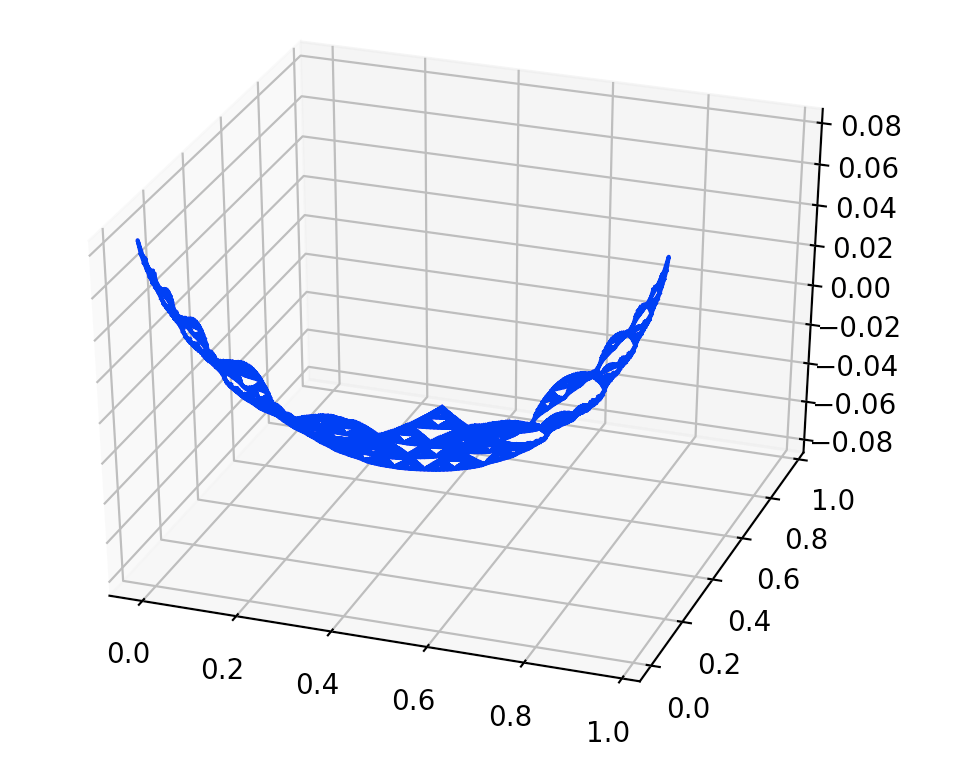
\includegraphics[width=.4\textwidth]{images/chebyshev_p11_0_0833.png}
    \caption{Plot of Chebyshev polynomial of order $1$ of family $1$, with $a=-\frac{1}{12}$. The boundary node on the left is $q_{1}$, the one on the right is $q_{2}$, and the boundary node on the back is 
    $q_{0}$.}
    \end{figure}
\end{frame}

\begin{frame}{Partial Results on $\mathcal{H}_1$}
    \begin{itemize}
        \item For the $2^{nd}$ Chebyshev polynomials of family $2$ and the family $3$, we only have experimental result, and our experiments show that $a_{2} = −0.0619339$ and $a_{3} = −0.0275013$
        \item We found those values by firstly determining loose bounds of $a_{2}$ and $a_{3}$, which are $[-\frac{2\beta_{1}}{\beta_{0}}, 0]=[-\frac{8}{45}, 0]$ for $a_{2}$ and $[-\frac{2\alpha_{1}}{\alpha_{0}}, 0]=[-\frac{1}{15}, 0]$ for $a_{3}$.
        \item Then we partition the intervals, test out each $a_{k}$, and look for the $a_{k}$ that gives the smallest uniform norm.
   \end{itemize}
\end{frame}

\begin{frame}{Image of $T_{12}(x)$}
    \begin{figure}[H]
    \centering
    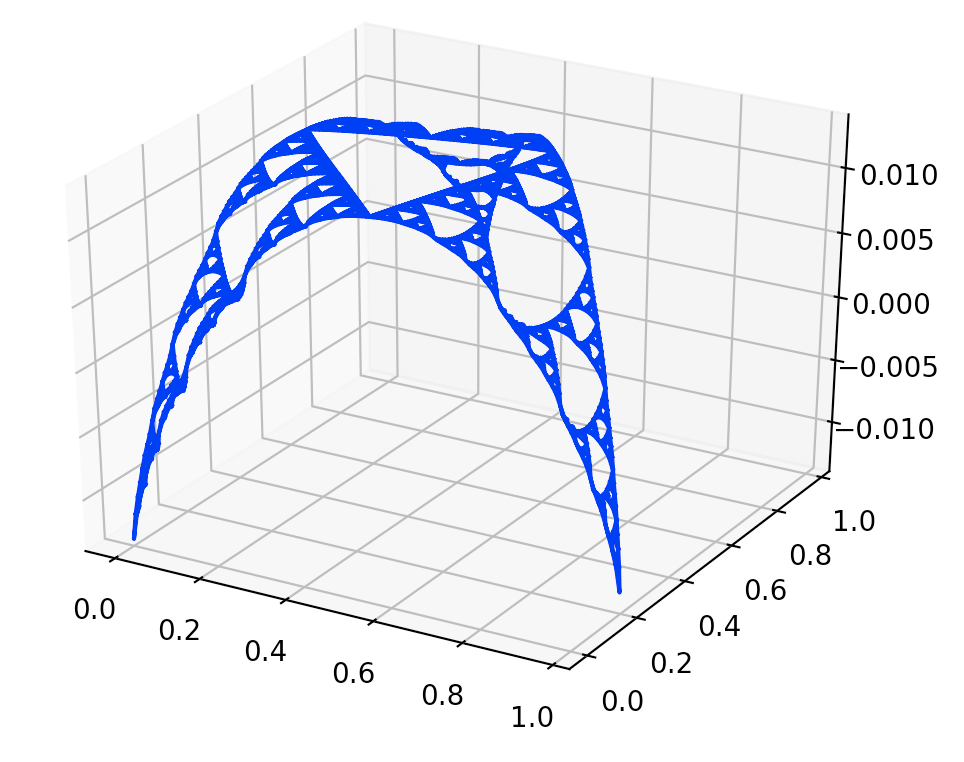
\includegraphics[width=.4\textwidth]{images/chebyshev_p12_0_0619339.png}
    \caption{Plot of Chebyshev polynomial of order $1$ of family $2$, with $a\approx -0.0619339$. The boundary node on the left is $q_{1}$, the one on the right is $q_{2}$, and the hidden boundary node on the back is $q_{0}$.}
    \end{figure}
\end{frame}

\begin{frame}{Image of $T_{13}(x)$}
    \begin{figure}[H]
    \centering
    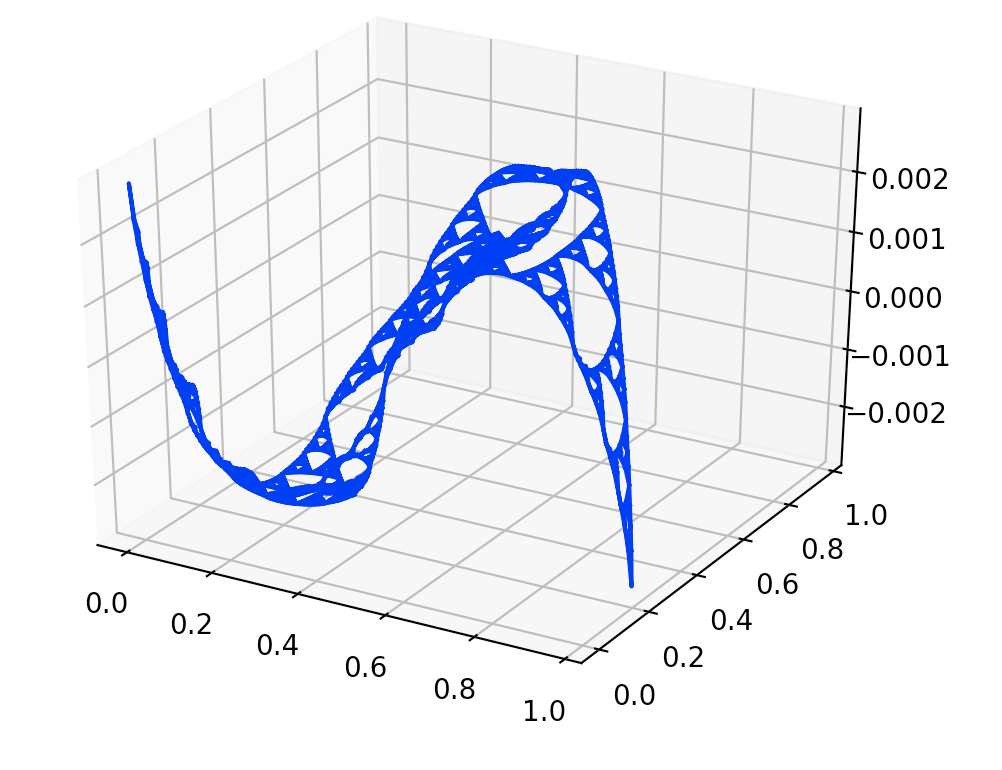
\includegraphics[width=.4\textwidth]{images/chebyshev_p13_0_02750235.png}
    \caption{Plot of Chebyshev polynomial of order $1$ of family $3$, with $a\approx -0.02750235$. The boundary node on the left is $q_{1}$, the one on the right is $q_{2}$, and the hidden boundary node on the back is $q_{0}$.}
    \end{figure}
\end{frame}

\begin{frame}{Alternating Property of Chebyshev Polynomials}
    \begin{itemize}
        \item A degree $n$ polynomial $P_{n}(x)$ defined on a compact set $K \subseteq \mathbb{R}$, has \textbf{an alternating set}, if $\exists \{x_{j}\}_{j=0}^n$ with $x_{0} < x_{1} < ...< x_{n}$, so that $P_{n}(x_{j}) = (-1)^{n-j}||P_{n}(x)||_{u}$.
        \item \textbf{The Alternation Theorem}: A monic polynomial of degree n is the Chebyshev polynomial if and only if it has an alternating set.
        \item The experimental results also show that the absolute value of the minimum and the maximum of the monic polynomials become closer when $a_{2}$ and $a_{3}$ approach the values that minimize their uniform norms.
    \end{itemize}
\end{frame}

\begin{frame}{Alternating Property of Chebyshev Polynomials}
    \begin{itemize}
        \item Assume that there exist an $a$, such that $Q(x) := P_{13}(x)+aP_{03}(x)$ achieves maximum norm at two distinct points $y \in \bigcup\limits_{m=0}^{\infty} F_{0}^{m}F_{1}SG$ and $z \in \bigcup\limits_{m=0}^{\infty} F_{0}^{m}F_{1}SG$, and $z = -y$. Then $Q(x)$ is the $1^{st}$ Chebyshev polynomial of the 3-family.
    
        \item Assume $Q(x)$ is not the first Chebyshev polynomial of the 3-family. Then $||T_{13}||_{\infty} < ||Q||_{\infty}$. This implies that $|T_{13}(x)| < |Q(x)|$ at $y$ and $z$. Thus $T_{13} - Q(x)$ cannot be both positive or negative at $y$ and $z$. Since both $T_{13}(x)$ and $Q(x)$ are monic, $T_{13} - Q(x)$ is spanned by $P_{03}$, and hence $T_{13} - Q(x)$ has to be both positive or negative at $y$ and $z$. We have a contradiction.
    \end{itemize}
\end{frame}

\begin{frame}{Further Questions}
    \begin{itemize}
        \item Find explicit formulas for Chebyshev polynomials of any degree.
        \item Replicate the alternation theorem to polynomials on SG.
        \item Study the orthogonality.
        \item Find the recurrence relation, if any.
    \end{itemize}
\end{frame}

\section{References}
\begin{frame}{References}
\begin{figure}
    \centering
    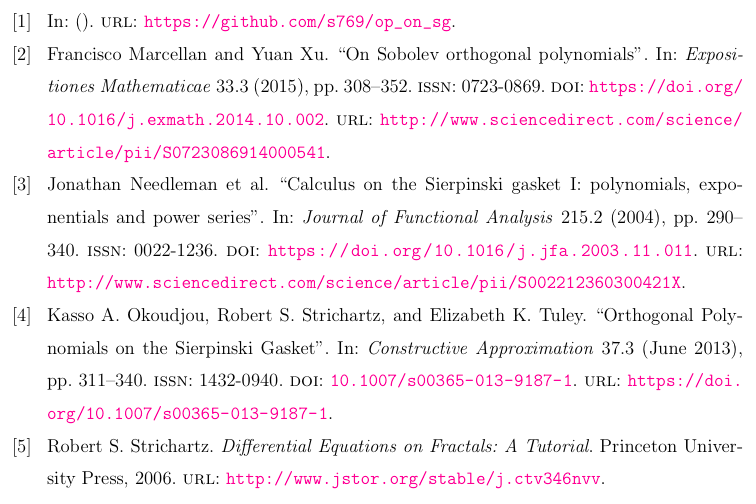
\includegraphics[width=0.95\linewidth]{Final_presentation/images/references.png}
 
    \label{fig:refs}
\end{figure}
\end{frame}
\begin{frame}{Questions?}
    \begin{figure}[H]
        \centering
        
\includegraphics[width=.7\textwidth]{images/meme.jpg}
        \label{fig:meme}
    \end{figure}
\end{frame}


% The theory of Sobolev orthogonal polynomials on $\mathbb{R}$ is well known and has gathered interest over the last 20 years. We build on this body of work by defining a Sobolev inner product on the Sierpinski Gasket and studying the corresponding Sobolev orthogonal polynomials. We find recurrence relations in the sequences of these polynomials and study their finer properties such as their $L^2$, $L^\infty$ and $H^1$ norms. We also use the Sobolev orthogonal polynomials to further understand the question around polynomial interpolation. Finally, we study the analogues of the Chebyshev polynomials and present some preliminary results and background related to them. 
\end{document}
